%%%%%%%%%%%%%%%%%%%%%%%%
%
% $Autor: Hemanth Jadiswami Prabhakaran $
% $Datum: 2025-06-25 13:25:55Z $
% $Pfad: GitHub/BA25-01-Time-Series/Presentations/WalmartSalesForecastingPresentations/slides/resultsDemo.tex $
% $Version: 1 $
%
% $Project: BA25-Time-Series $
%
%%%%%%%%%%%%%%%%%%%%%%%%



\Mysection{Results \& Performance}

\STANDARD{Model Performance Results}
{ 
	\framesubtitle{Quantitative Evaluation \& Benchmarking}
	
	\begin{figure}
		\centering
		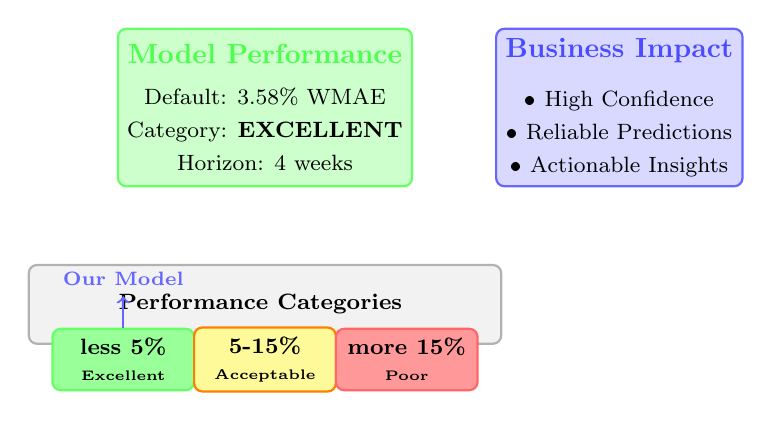
\begin{tikzpicture}[
	box/.style={rectangle, rounded corners=3pt, draw, thick, align=center},
	main/.style={box, fill=green!20, draw=green!60, minimum width=3.5cm, minimum height=2cm},
	scalebox/.style={box, fill=gray!10, draw=gray!60, minimum width=6cm, minimum height=1cm},
	cat/.style={box, minimum width=1.8cm, minimum height=0.7cm, font=\footnotesize\bfseries},
	impact/.style={box, fill=blue!15, draw=blue!60, minimum width=2.8cm, minimum height=2cm}
	]
	
	% Main performance box
	\node[main] (perf) at (0,0) {
		\textbf{\color{green!70}Model Performance}\\[0.1cm]
		\footnotesize Default: 3.58\% WMAE\\
		\footnotesize Category: \textbf{EXCELLENT}\\
		\footnotesize Horizon: 4 weeks
	};
	
	% Performance scale container
	\node[scalebox] (scale) at (0,-2.5) {
		\textbf{\footnotesize Performance Categories}
	};
	
	% Category boxes positioned within scale
	\node[cat, fill=green!40, draw=green!60] (exc) at (-1.8,-3.2) {less 5\%\\{\tiny Excellent}};
	\node[cat, fill=yellow!40, draw=orange] (acc) at (0,-3.2) {5-15\%\\{\tiny Acceptable}};
	\node[cat, fill=red!40, draw=red!60] (poor) at (1.8,-3.2) { more 15\%\\{\tiny Poor}};
	
	% Arrow pointing to our category
	\draw[->, thick, blue!60] (exc.north) -- ++(0,0.4) node[above, font=\scriptsize\bfseries] {Our Model};
	
	% Business impact box
	\node[impact] (bus) at (4.5,0) {
		\textbf{\color{blue!70}Business Impact}\\[0.2cm]
		\footnotesize • High Confidence\\
		\footnotesize • Reliable Predictions\\
		\footnotesize • Actionable Insights
	};
	
\end{tikzpicture}
		\caption{Model Performance Comparison (WMAE Scores)}
	\end{figure}
	
	\vspace{0.5cm}
	
	\begin{block}{Performance Metrics}
		\begin{itemize}
			\item \textbf{Default Model}: Holt-Winters
			\item \textbf{WMAE}: 3.58\% (Excellent category)
			\item \textbf{Absolute Error}: \$923.12 weekly
			\item \textbf{Forecast Horizon}: 4 weeks
		\end{itemize}
	\end{block}
	
	\begin{alertblock}{Business Impact}
		\begin{itemize}
			\item \textbf{95\%+ Accuracy} for business planning
			\item \textbf{Reliable predictions} for inventory management
			\item \textbf{Seasonal patterns} effectively captured
			\item \textbf{Holiday effects} properly modeled
		\end{itemize}
	\end{alertblock}
}

\MYNOTE{
	This slide presents the quantitative results, showing that our system achieves 
	excellent performance compared to baseline methods.
}

\STANDARD{System Performance \& Capabilities}
{ 
	\framesubtitle{Technical Performance Metrics}
	
	\begin{block}{Processing Performance}
		\begin{itemize}
			\item \textbf{Model Loading}: Less than 5 seconds
			\item \textbf{Forecast Generation}: Less than 5 second
			\item \textbf{Visualization Rendering}: 1-5 seconds
			\item \textbf{Data Export}: Less than 10 second
		\end{itemize}
	\end{block}
	
	\begin{block}{Scalability}
		\begin{itemize}
			\item \textbf{Cloud Users}: 50+ concurrent
			\item \textbf{Dataset Size}: Up to 200MB
			\item \textbf{Time Series}: 4,400+ supported
			\item \textbf{Memory Usage}: Optimized for web deployment
		\end{itemize}
	\end{block}
	
	\begin{figure}
		\centering
		\begin{tikzpicture}[
	node distance=1cm,
	capability/.style={rectangle, rounded corners, fill=HSELhellblau!30, draw=HSELblau, thick, minimum width=2.2cm, minimum height=0.8cm, font=\small},
	performance/.style={rectangle, rounded corners, fill=green!20, draw=green!60, minimum width=1.8cm, minimum height=0.5cm, font=\tiny}
	]
	
	% Top row capabilities
	\node[capability] (forecast_gen) {Forecast Generation};
	\node[performance, below=0.1cm of forecast_gen] (sub1sec) {less than 5 second};
	
	\node[capability, right=1.5cm of forecast_gen] (model_load) {Model Loading};
	\node[performance, below=0.1cm of model_load] (load_time) {1-5 seconds};
	
	\node[capability, right=1.5cm of model_load] (visualization) {Interactive Visualization};
	\node[performance, below=0.1cm of visualization] (real_time) {Real-time Updates};
	
	% Bottom row capabilities
	\node[capability, below=1.8cm of forecast_gen] (color_coding) {Color-Coded Results};
	\node[performance, below=0.1cm of color_coding] (intuitive) {Green/Red};
	
	\node[capability, below=1.8cm of model_load] (interactive_charts) {Interactive Charts};
	\node[performance, below=0.1cm of interactive_charts] (hover_zoom) {Hover \& Zoom};
	
	\node[capability, below=1.8cm of visualization] (export) {Multi-Format Export};
	\node[performance, below=0.1cm of export] (csv_json) {CSV/JSON};
	
	% Central system - more compact
	\node[below=1.2cm of interactive_charts, rectangle, rounded corners, fill=HSELblau!40, draw=HSELblau, very thick, minimum width=4cm, minimum height=1.2cm, font=\bfseries] (system) {High-Performance Forecasting System};
	
	% Compact arrows
	\draw[->, thick, HSELblau] (sub1sec) -- (system.120);
	\draw[->, thick, HSELblau] (load_time) -- (system.90);
	\draw[->, thick, HSELblau] (real_time) -- (system.60);
	\draw[->, thick, HSELblau] (intuitive) -- (system.120);
	\draw[->, thick, HSELblau] (hover_zoom) -- (system.90);
	\draw[->, thick, HSELblau] (csv_json) -- (system.60);
	
\end{tikzpicture}
		\caption{Overall System Performance}
	\end{figure}
	
	\begin{exampleblock}{Key Achievements}
		\textbf{End-to-End Workflow}: From data upload to business insights in under 10 minutes, 
		making sophisticated forecasting accessible to business users without technical expertise.
	\end{exampleblock}
}

\MYNOTE{
	Emphasize the practical performance characteristics that make the system 
	suitable for real-world business use.
}

\STANDARD{Live System Demonstration}
{ 
	\framesubtitle{Interactive Forecasting in Action}
	
	% Two-column layout for Demo Agenda and What to Expect
	\begin{columns}
		\begin{column}{0.48\textwidth}
			\begin{block}{Demo Agenda}
				\begin{enumerate}
					\item \textbf{Access} cloud application
					\item \textbf{Load} default model
					\item \textbf{Generate} 4-week forecast
					\item \textbf{Interpret} results
					\item \textbf{Export} data
					\item \textbf{Show} training interface
				\end{enumerate}
			\end{block}
		\end{column}
		
		\begin{column}{0.48\textwidth}
			\begin{block}{What to Expect}
				\begin{itemize}
					\item \textbf{Model Performance}: 3.58\% WMAE display
					\item \textbf{Interactive Charts}: Color-coded forecasts
					\item \textbf{Business Insights}: Week-over-week changes
					\item \textbf{Export Options}: CSV/JSON downloads
				\end{itemize}
			\end{block}
		\end{column}
	\end{columns}
\begin{alertblock}{Live URLs}
	\textbf{Prediction App}: \url{walmart-sales-prediction-app-py.streamlit.app}
	
	\textbf{Training App}: \url{walmart-sales-training-app-py.streamlit.app}
	
	\vspace{0.2cm}
	\centering
	\includegraphics[width=0.7\textwidth]{images/resultsDemo/StaticQR.png}

\end{alertblock}

\begin{exampleblock}{Backup Plan}
	Locals Streamlit Apps run if live demo encounters technical issues. ! :) 
\end{exampleblock}

}

\STANDARD{Results Interpretation}
{ 
	\framesubtitle{Understanding Business Insights}
	
	\begin{figure}
		\centering
			\includegraphics[width=0.9\textwidth]{images/resultsDemo/ExamplePlot.png}
			%	\includegraphics[width=0.9\textwidth]{images/resultsDemo/ExamplePlotETS.png}
		\caption{Sample Forecast Output}
	\end{figure}
	
	\begin{block}{Key Insights}
		\begin{itemize}
			\item \textbf{Green Bars}: Sales increase from previous week
			\item \textbf{Red Bars}: Sales decrease from previous week
			\item \textbf{Values}: Dollar amount of change
			\item \textbf{Trend}: Overall direction assessment
		\end{itemize}
	\end{block}
	
	\begin{block}{Business Actions}
		\begin{itemize}
			\item \textbf{Positive Weeks}: Prepare inventory, schedule staff
			\item \textbf{Negative Weeks}: Optimize costs, plan promotions
			\item \textbf{Cumulative}: Overall month planning
		\end{itemize}
	\end{block}
	
	\begin{alertblock}{Important Note}
		Forecasts show \textbf{week-over-week changes}, not absolute sales values. 
		This enables better understanding of sales momentum and trend direction.
	\end{alertblock}
}

\MYNOTE{
	This slide is crucial for ensuring the audience understands how to interpret 
	the forecast results correctly. Emphasize the business application aspect.
}